\section{Experiments and Results}
\label{sec:experiments}

\subsection{Comparison of Architectures}
\label{subsec:arch_compare}

We benchmark a wide range of lightweight and efficient architectures on the AvocadoLeaf test set. Table~\ref{tab:arch_compare} reports top-1 accuracy, macro F1 score, number of parameters, and per-image inference time on a single NVIDIA RTX 3050-6GB GPU for all 15 evaluated models. All models share the same optimiser, learning-rate schedule, and data augmentation policy (Section~\ref{sec:proposed_model}). Each architecture was trained once (single seed); to account for the uncertainty this and the finite 280-image test set introduce, we additionally report bootstrap 95\% confidence intervals and paired significance tests in \ref{app:bootstrap}.

\begin{table*}[t]
\centering
\caption{Performance comparison of all evaluated architectures. The highest values in each column are highlighted in bold and underlined.}
\label{tab:arch_compare}
\small
\setlength{\tabcolsep}{3pt}
\begin{tabularx}{\textwidth}{X c c c c}
\toprule
\textbf{Model} & \makecell[c]{\textbf{Acc}\\(\%)} & \makecell[c]{\textbf{Macro F1}} & \makecell[c]{\textbf{Params}\\(M)} & \makecell[c]{\textbf{Inference}\\(ms)} \\
\midrule
ConvNeXt-V2            & \textbf{\underline{92.14}} & 0.900 &  3.4 & 2.30 \\
SwinTransformer        & 91.43 & 0.899 & 27.5 & 6.69 \\
MobileOne              & 91.43 & 0.893 &  4.3 & 8.35 \\
ConvNeXt-V1            & 91.07 & 0.895 & 27.8 & 5.24 \\
ViT                    & 91.07 & \textbf{\underline{0.904}} & 85.8 & 14.25 \\
EdgeNeXt               & 91.07 & 0.877 &  5.3 & 3.75 \\
ResNet-18              & 88.93 & 0.863 & 11.2 & 1.98 \\
TinyNet                & 88.21 & 0.863 &  4.9 & 3.66 \\
FastViT                & 87.50 & 0.853 &  3.3 & 3.63 \\
MobileNet-V2           & 87.14 & 0.847 &  2.2 & 1.80 \\
EfficientNet-B0        & 86.43 & 0.838 &  4.0 & 2.85 \\
MobileNet-V4           & 76.07 & 0.724 &  2.5 & 1.89 \\
EfficientViT           & 69.29 & 0.650 &  3.2 & 7.00 \\
GhostNet-V2            & 69.29 & 0.571 &  4.9 & 5.43 \\
VanillaCNN             & 63.57 & 0.623 & 25.8 & 1.33 \\
\bottomrule
\end{tabularx}
\end{table*}


Among the evaluated models, ConvNeXt-V2 achieves the highest point-estimate classification accuracy (92.14\%) and the second-highest macro F1 score (0.900), while maintaining a compact parameter count (3.4M) and low inference latency (2.30 ms). However, bootstrap significance testing (\ref{app:bootstrap}) shows that its accuracy advantage over the next five models (SwinTransformer, MobileOne, ViT, EdgeNeXt, and ConvNeXt-V1) is \emph{not} statistically significant at this test set size ($p > 0.5$ for all five); these six models should be regarded as statistically tied in accuracy. In particular, ViT attains the highest macro F1 (0.904) but has 85.8M parameters and requires 14.25 ms per inference, making it impractical for edge deployment despite its statistically indistinguishable accuracy. What separates ConvNeXt-V2 from the rest of this tied top group is not proven superior accuracy but a far smaller parameter count (3.4M vs. 4.3--85.8M for the other five) and lower latency, which is why we select it as our proposed lightweight model. ConvNeXt-V2's advantage over every model ranked sixth or lower \emph{is} statistically significant ($p < 0.05$, \ref{app:bootstrap}). Conversely, lightweight architectures such as MobileNet-V2 and EfficientNet-B0 are faster and smaller but lag significantly in accuracy (approximately 86–87\%), which is insufficient for reliable field diagnosis. Models with accuracy below 80\% (MobileNet-V4, EfficientViT, GhostNet-V2, VanillaCNN) lack the representational capacity required for this fine-grained classification task. Overall, ConvNeXt-V2 offers the most favourable balance among accuracy, model size, and speed, making it the strongest candidate among the evaluated architectures for deployment on resource-constrained devices, pending on-device latency validation (Section~\ref{sec:discussion}).

To further understand the impact of model capacity, we group the 14 fine-tuned, ImageNet-pretrained architectures into two categories, including (1) \textit{lightweight models} with fewer than 5 million parameters (9 models) and (2) \textit{heavy models} with 5 million or more (5 models). The VanillaCNN baseline is excluded from this comparison: its 25.8M parameter count reflects an unoptimised from-scratch architecture rather than a deliberate heavy-model design choice, and including it by parameter count alone would place a 0.623 F1 score inside the heavy group purely as an artefact of training regime, not capacity. The heavy group achieves a high and stable mean F1 of 0.888, with all models scoring above 0.86. The light group shows much greater variance, with a mean of 0.793 and scores ranging from 0.571 to 0.900. 
ConvNeXt-V2 stands out as the only light model attaining F1 (0.900) comparable to the best heavy architectures while using substantially fewer parameters. This confirms that model selection is critical under parameter constraints, whereas heavy models offer stable performance at the cost of larger size and slower inference. 
\begin{figure}[htbp]
\centering
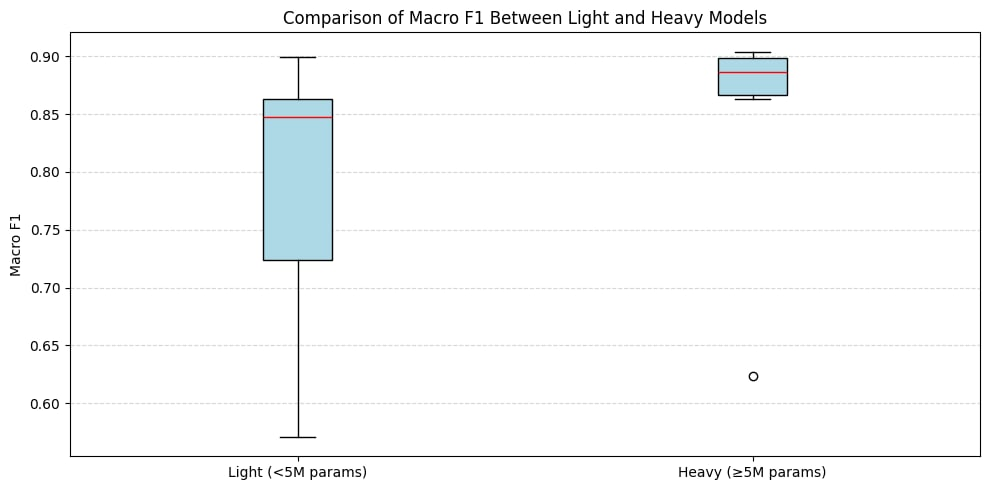
\includegraphics[width=\columnwidth]{img/models/f1_comparision.jpg}
\caption{Macro F1 scores of all evaluated models. Lightweight models (<5M parameters) are shown in blue, heavy models ($\geq$5M) in orange.}
\label{fig:f1_comparision}
\end{figure}


\subsubsection{Efficiency Analysis}
\label{subsec:efficiency}

To jointly assess accuracy, model size, and inference speed, we define a composite efficiency metric:

\[
\text{Efficiency} = \frac{\text{Macro F1}}{\text{Params (M)} \times \text{Inference Time (ms)}}.
\]

This metric quantifies the predictive performance achieved per unit of resource consumption, where higher values indicate better trade-offs among the three dimensions. Figure~\ref{fig:efficiency} visualises two complementary efficiency dimensions, F1 per million parameters (F1/Params) and F1 per millisecond inference time (F1/Time); the colour scale indicates macro F1.

\begin{figure}[htbp]
\centering
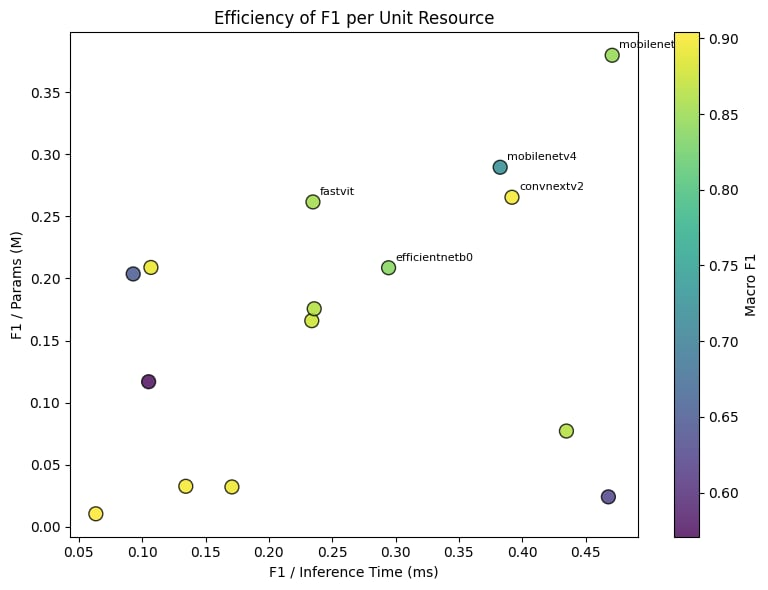
\includegraphics[width=\columnwidth]{img/models/efficiency.jpg}
\caption{Scatter plot of F1 per parameter versus F1 per inference time. Colour indicates macro F1.}
\label{fig:efficiency}
\end{figure}

MobileNet-V2 achieves the highest overall efficiency (0.211) due to its extremely compact size (2.2M parameters) and fast inference (1.80 ms), though its macro F1 (0.847) is moderate. ConvNeXt-V2 ranks third in efficiency (0.116) while attaining a substantially higher F1 (0.900). Its F1/Params (0.265) and F1/Time (0.391) are well balanced, placing it in the upper-right region of the scatter plot. Heavy models such as ViT (0.001) and SwinTransformer (0.005) exhibit very low efficiency despite competitive F1, due to large parameter counts and slower inference. These results indicate that ConvNeXt-V2 offers the most favourable balance between accuracy and resource utilisation among the evaluated architectures, based on parameter count and GPU inference latency.

\subsubsection{Ablation Study}
\label{subsec:ablation}

To isolate the contribution of two training-protocol switches exposed by our pipeline, namely data augmentation and class-weighted loss, we retrain Model BoVien (ConvNeXt-V2) under all four combinations, holding the architecture, optimiser, schedule, and epoch budget fixed. This does not repeat the full 15-architecture sweep; it only probes the proposed model itself. Each configuration is again trained once (single seed) on the same 280-image test set, so, following the same protocol as Section~\ref{subsec:arch_compare}, we report bootstrap 95\% confidence intervals and paired significance tests in \ref{app:bootstrap_ablation}.

\begin{table}[htbp]
\centering
\caption{Ablation of augmentation and class-weighted loss on Model BoVien (AvocadoLeaf test set).}
\label{tab:ablation}
\small
\begin{tabularx}{\columnwidth}{X c c}
\toprule
\textbf{Configuration} & \textbf{Acc (\%)} & \textbf{Macro F1} \\
\midrule
No augmentation, no class-weight   & \textbf{\underline{92.14}} & \textbf{\underline{0.900}} \\
No augmentation, class-weighted    & 90.71 & 0.887 \\
Augmentation, no class-weight      & 88.93 & 0.864 \\
Augmentation, class-weighted       & 91.43 & 0.895 \\
\bottomrule
\end{tabularx}
\end{table}

\begin{figure}[htbp]
\centering
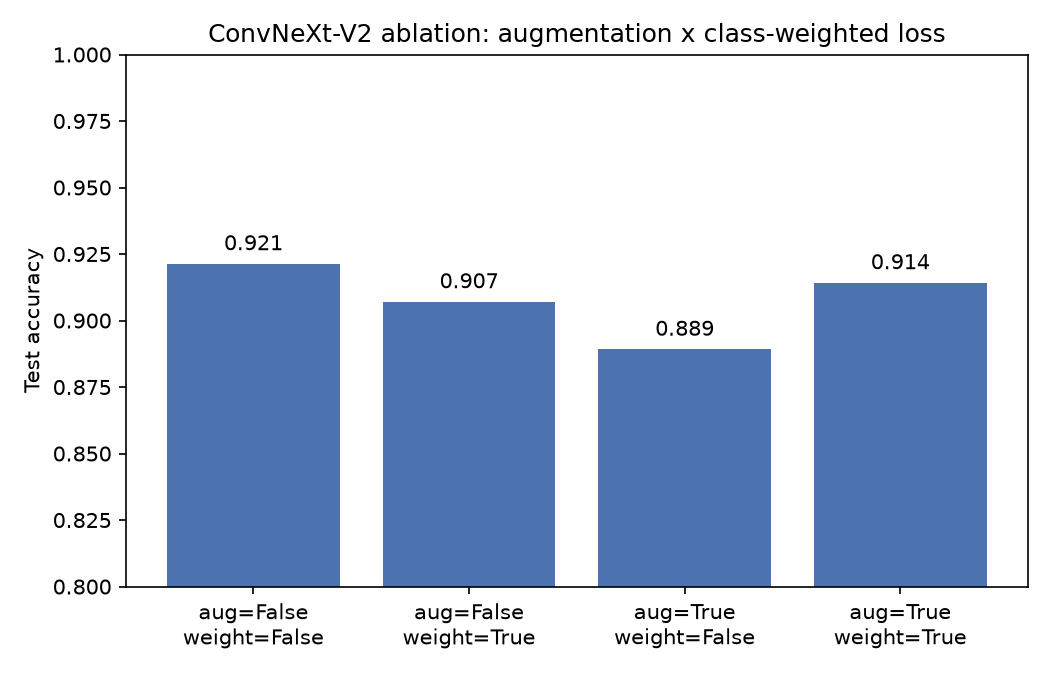
\includegraphics[width=\columnwidth]{img/experiments/ablation/ablation_accuracy.png}
\caption{Test accuracy of Model BoVien under the four augmentation $\times$ class-weighted-loss combinations.}
\label{fig:ablation}
\end{figure}

The no-augmentation, no-class-weight configuration is the best of the four, and its accuracy (92.14\%) matches the ConvNeXt-V2 row of Table~\ref{tab:arch_compare} exactly. This ablation grid includes the very checkpoint reported as our proposed model, not a separately retrained approximation of it, and confirms that the reported BoVien checkpoint was trained \emph{without} augmentation. This differs from the augmentation policy described in Section~\ref{sec:proposed_model}, which we flag as a documentation/protocol discrepancy in Section~\ref{sec:discussion} rather than silently reconcile here. Adding augmentation alone costs 3.2 accuracy points (92.14\% $\to$ 88.93\%), the largest single-factor drop in the grid, and adding class-weighting on top of augmentation recovers about two-thirds of that loss (88.93\% $\to$ 91.43\%) but still falls short of the no-augmentation baseline. Class-weighting alone also underperforms the plain baseline, though by a smaller margin (92.14\% $\to$ 90.71\%). A plausible explanation for augmentation hurting this particular model is that, on AvocadoLeaf's comparatively small training set (1,302 images), the added geometric and photometric perturbations remove information that ConvNeXt-V2's frozen-backbone-plus-fine-tuned-stages setup would otherwise use productively, though this ablation grid alone cannot rule out that the same holds for the other 14 candidate architectures. However, bootstrap significance testing (\ref{app:bootstrap_ablation}) shows that none of these three differences are statistically significant at this test set size, including the largest one (no augmentation, no class-weight, versus augmentation, no class-weight, $+$3.31pp, $p = 0.054$); the ranking above should therefore be read as suggestive rather than conclusive, consistent with how Section~\ref{subsec:arch_compare}'s single-seed, 280-image comparisons are treated throughout this paper.

\subsubsection{Error Analysis}
\label{subsec:error_analysis}

To characterise \emph{which} classes drive the remaining test-set errors, rather than only the aggregate 92.14\% figure, we re-examine BoVien's 280 per-image test predictions (already saved by the evaluation pipeline; no re-inference) through its confusion matrix.

\begin{figure}[htbp]
\centering
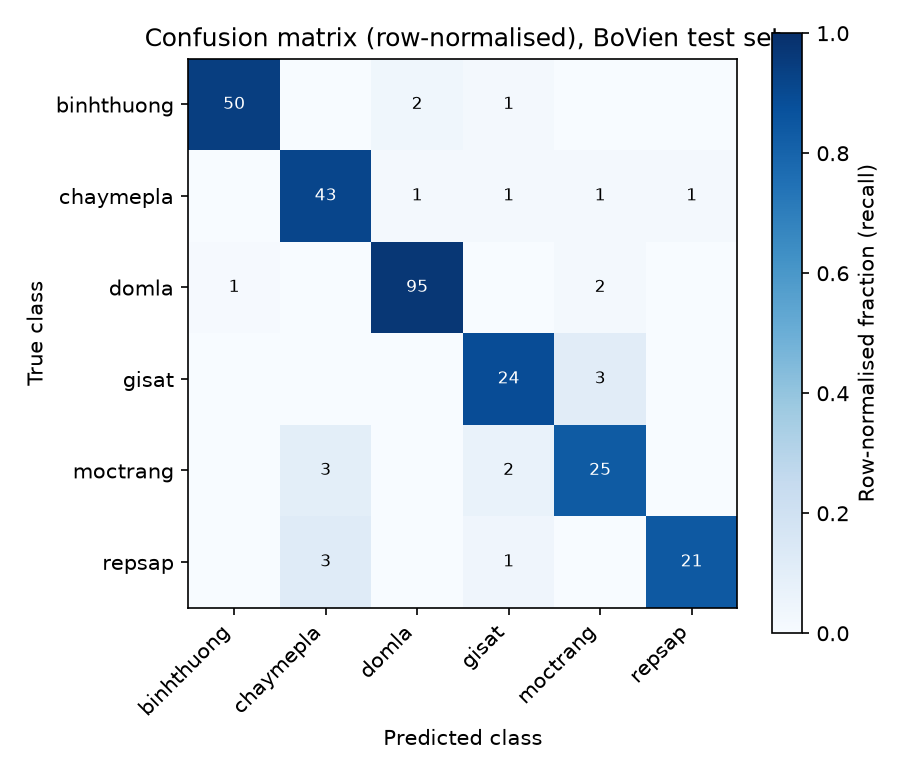
\includegraphics[width=\columnwidth]{img/experiments/evaluating/confusion_matrix_heatmap.png}
\caption{Row-normalised confusion matrix (raw counts annotated) for Model BoVien on the AvocadoLeaf test set.}
\label{fig:confusion_matrix}
\end{figure}

Per-class recall ranges from 96.9\% (\textit{domla}, the largest class at 458 training images) down to 83.3--84.0\% for the three smallest classes, \textit{moctrang} (136 training images, 83.3\% recall), \textit{repsap} (115, 84.0\%), and \textit{gisat} (128, 88.9\%), while the three larger classes (\textit{domla} 458, \textit{binhthuong} 245, \textit{chaymepla} 220) all exceed 91\% recall. This is consistent with a straightforward sample-size effect rather than any one class being intrinsically harder to photograph or define. The confusions are concentrated in three symmetric pairs: \textit{gisat} (algal leaf spot, orange velvety pustules) $\leftrightarrow$ \textit{moctrang} (powdery mildew, white powdery coating) account for 5 of 280 errors in both directions, \textit{repsap} (mealybug damage, silver/stippled marks) is confused with \textit{chaymepla} (leaf scorch, margin/tip burn) in 12.0\% of \textit{repsap} images, and \textit{moctrang} is likewise confused with \textit{chaymepla} in 10.0\% of its images. All three pairs share a plausible visual explanation: each involves a diffuse or patchy discolouration (algal spots, powdery coating, insect stippling) that can visually resemble scorch damage or a different spot pattern under variable field lighting, rather than the compact, high-contrast lesions of \textit{domla}. Notably, \textit{repsap} is also the class with the lowest LIME faithfulness score (Section~\ref{subsec:interpretability}, mean confidence drop 0.416 vs.\ 0.649 overall), so its diffuse, non-contiguous damage pattern appears to make it both harder to classify correctly and harder to explain with a fixed-size superpixel mask, two independent pieces of evidence pointing at the same underlying cause. Full per-class and per-pair breakdowns are in \texttt{deliverables/evaluating/\{per\_class\_error\_summary,confused\_pairs\}.csv}.

\subsection{Model Interpretability}
\label{subsec:interpretability}

To assess whether ConvNeXt‑V2 relies on disease‑relevant visual evidence rather than spurious correlations, we apply LIME \cite{ribeiro2016why} to every image in the 280-image test set (not merely a qualitative sample). Each image is segmented into superpixels with the Quickshift algorithm, and 500 perturbed samples are used to fit a local surrogate model that identifies the superpixels most responsible for the predicted class.

We quantify faithfulness with a deletion metric. For each test image, we hide exactly the superpixels LIME identifies as most responsible for the predicted class (the same masking colour used during LIME's own perturbation sampling) and re-run the model, measuring how much its confidence in the predicted class drops. A faithful explanation should cause a large drop, since it claims the hidden region is what the prediction relies on. Averaged over all 280 test images, hiding the LIME-highlighted region (which covers only 20.0\% of the image area on average) drops the model's confidence in its own predicted class from 0.940 to 0.292, a mean confidence drop of 0.649 (bootstrap 95\% CI [0.618, 0.678], see \ref{app:lime_faithfulness} for the full methodology and per-class breakdown). The drop is larger for correctly classified images (0.660, $n=258$) than for misclassified ones (0.516, $n=22$), consistent with correct predictions being more strongly grounded in genuine symptomatic regions rather than spurious cues. This full-test-set quantitative result substantially strengthens the qualitative examples below.

Figure~\ref{fig:lime_examples} shows two representative qualitative examples. For \textit{chaymepla}, the highlighted superpixels tightly enclose the brown, scorched lesion at the centre of the leaf, closely matching the visible symptom boundary. For \textit{moctrang} (powdery mildew), the highlighted regions concentrate on the white powdery patches on the leaf surface rather than on the unaffected tissue or background. These qualitative results illustrate that ConvNeXt‑V2's predictions are driven by the same visual cues a human expert would use, rather than by background or imaging artefacts, consistent with the quantitative deletion-metric result above.

\begin{figure}[htbp]
\centering
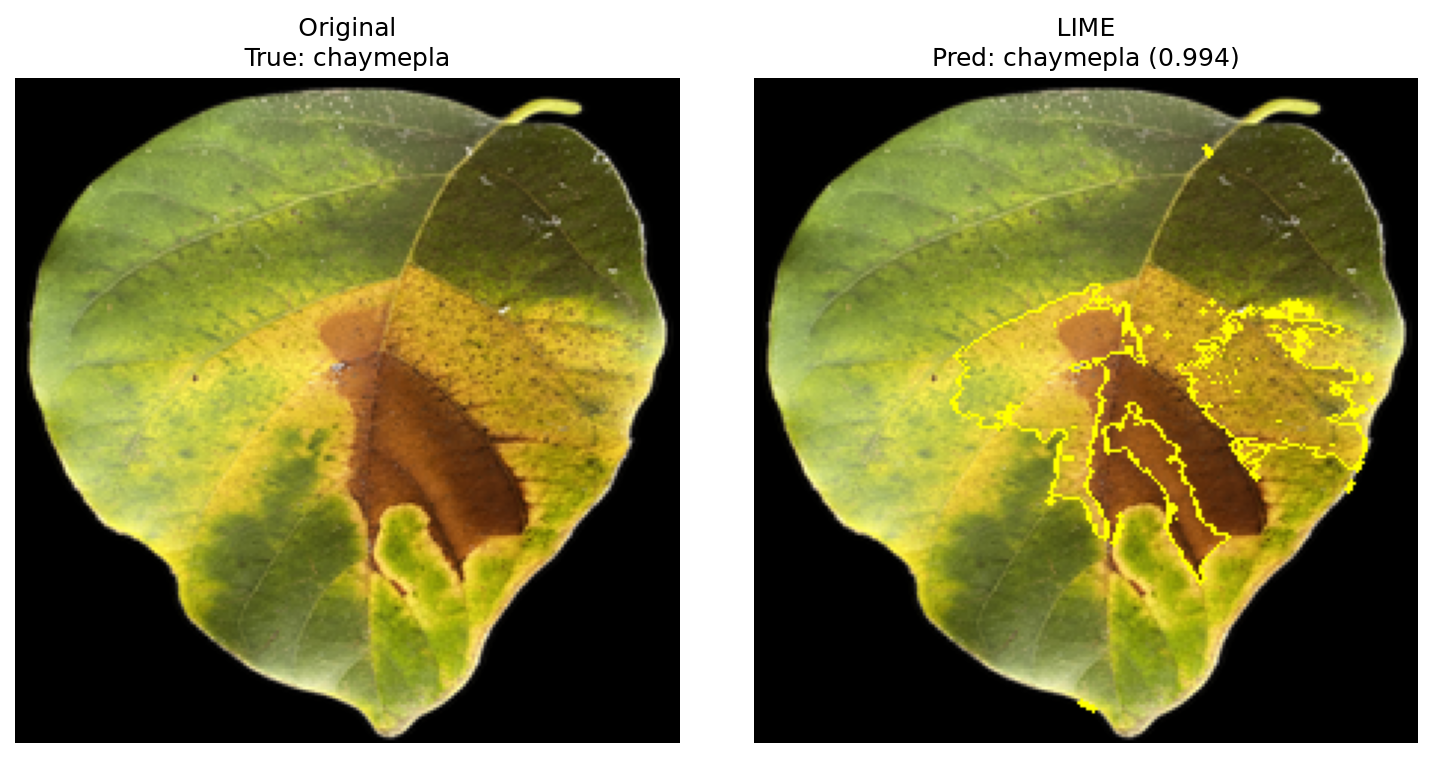
\includegraphics[width=0.49\linewidth]{img/experiments/xai/chaymepla_lime.png}
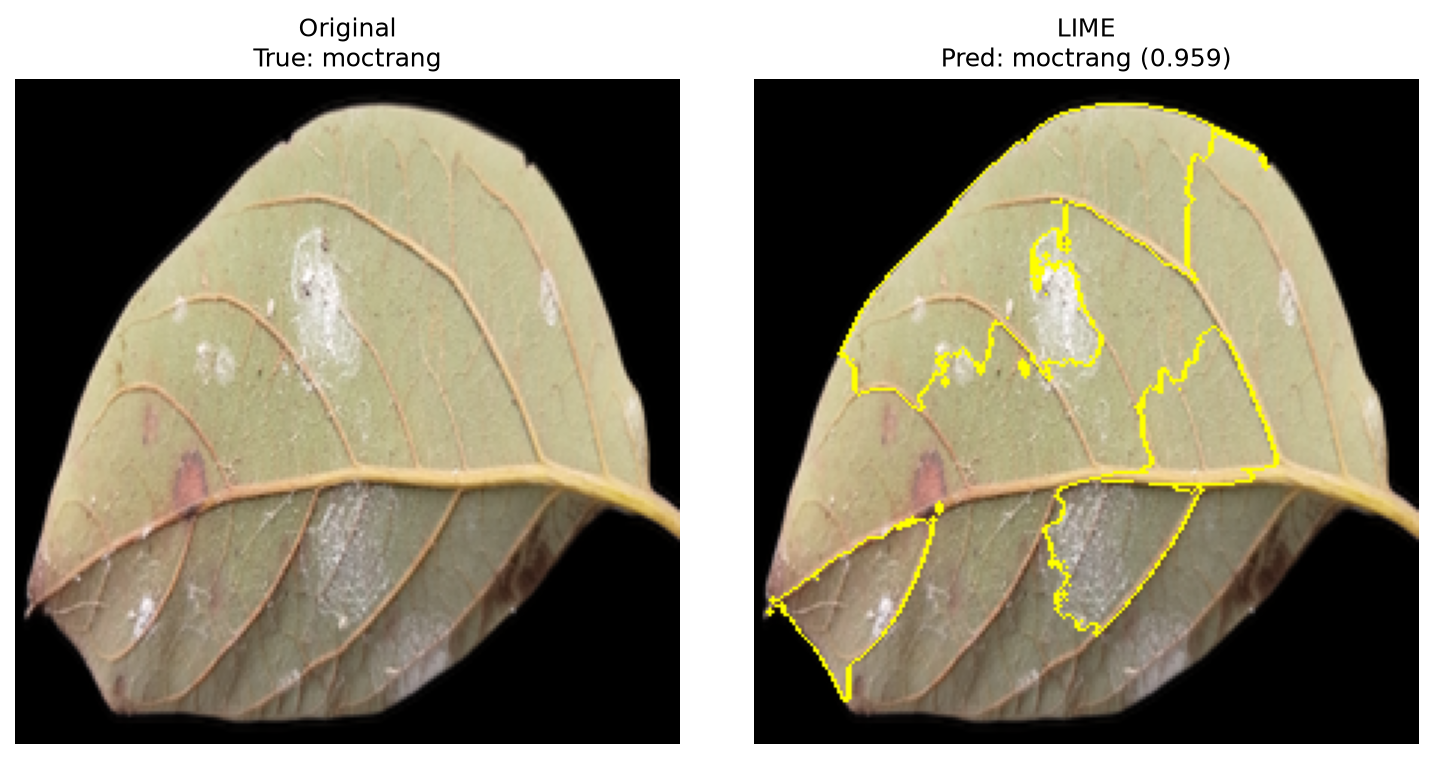
\includegraphics[width=0.49\linewidth]{img/experiments/xai/moctrang_lime.png}
\caption{LIME explanations for ConvNeXt‑V2 on two disease classes. Left, \textit{chaymepla} (leaf scorch), where the highlighted region matches the scorched lesion; right, \textit{moctrang} (powdery mildew), where the highlighted region matches the white powdery patches. Yellow outlines mark superpixels positively attributed to the predicted class.}
\label{fig:lime_examples}
\end{figure}

\subsection{Multi-modal Explanation Generation (CNN + LIME + VLM)}
\label{subsec:vlm_explain}

LIME identifies \emph{which pixels} a prediction depends on but produces no natural-language account of \emph{why} those pixels are diagnostically relevant, a gap that matters for a farmer-facing tool, where a highlighted region without a caption is of limited practical use. We therefore built a pipeline combining all three components developed in this work (the CNN's prediction, LIME's visual attribution, and a small, locally-hosted vision-language model, \texttt{Qwen2-VL-2B-Instruct}, no API cost) to generate a grounded natural-language explanation. Critically, the CNN remains the sole decision-maker. The VLM is given the CNN's already-decided class label together with the raw leaf image and the LIME overlay image, and is asked only to describe the visual evidence and judge whether it supports that label, never to propose a different one (\texttt{final\_pred} is verified to equal the CNN's prediction for 100\% of processed images). This design was applied to the 140 test images ConvNeXt‑V2 was least confident about (top 50\% by MC-Dropout predictive entropy).

Figure~\ref{fig:explain_vlm_showcase} shows three outputs of this pipeline, hand-selected from the 140-image escalated subset as coherent, correctly-grounded examples rather than a random or representative sample (full text in Table~\ref{tab:explain_vlm_showcase}). In these examples, the generated text correctly references both the LIME-highlighted location (e.g. ``vùng giữa hai lá'') and the specific visual symptom expected for the class (e.g. rust-coloured spots for \textit{gisat}, white powdery patches for \textit{moctrang}), demonstrating that the pipeline \emph{can} turn a raw prediction and an attribution map into an interpretable, farmer-readable statement, which was the original motivation for adding a language model to this system. Not every generated explanation is this coherent, however; Section~\ref{sec:discussion} discusses a case where the model's reasoning conflated the symptom description of a different class.

Across the full 140-image escalated subset, the VLM judged the visual evidence to support the CNN's diagnosis for 92.0\% of the 125 images that produced a parseable response. This figure should not be read as a validated accuracy or quality score; it is simply how often the model answered ``yes'', and it is in fact somewhat higher than ConvNeXt‑V2's own 85.0\% accuracy on this same subset (\ref{app:llm}). This is consistent with the low recall (0.21) for detecting actual mistakes reported in Section~\ref{sec:discussion}, as the model agrees with the CNN more often than the CNN is actually correct, suggesting a degree of acquiescence bias rather than critical evaluation of the evidence.

\begin{figure}[htbp]
\centering
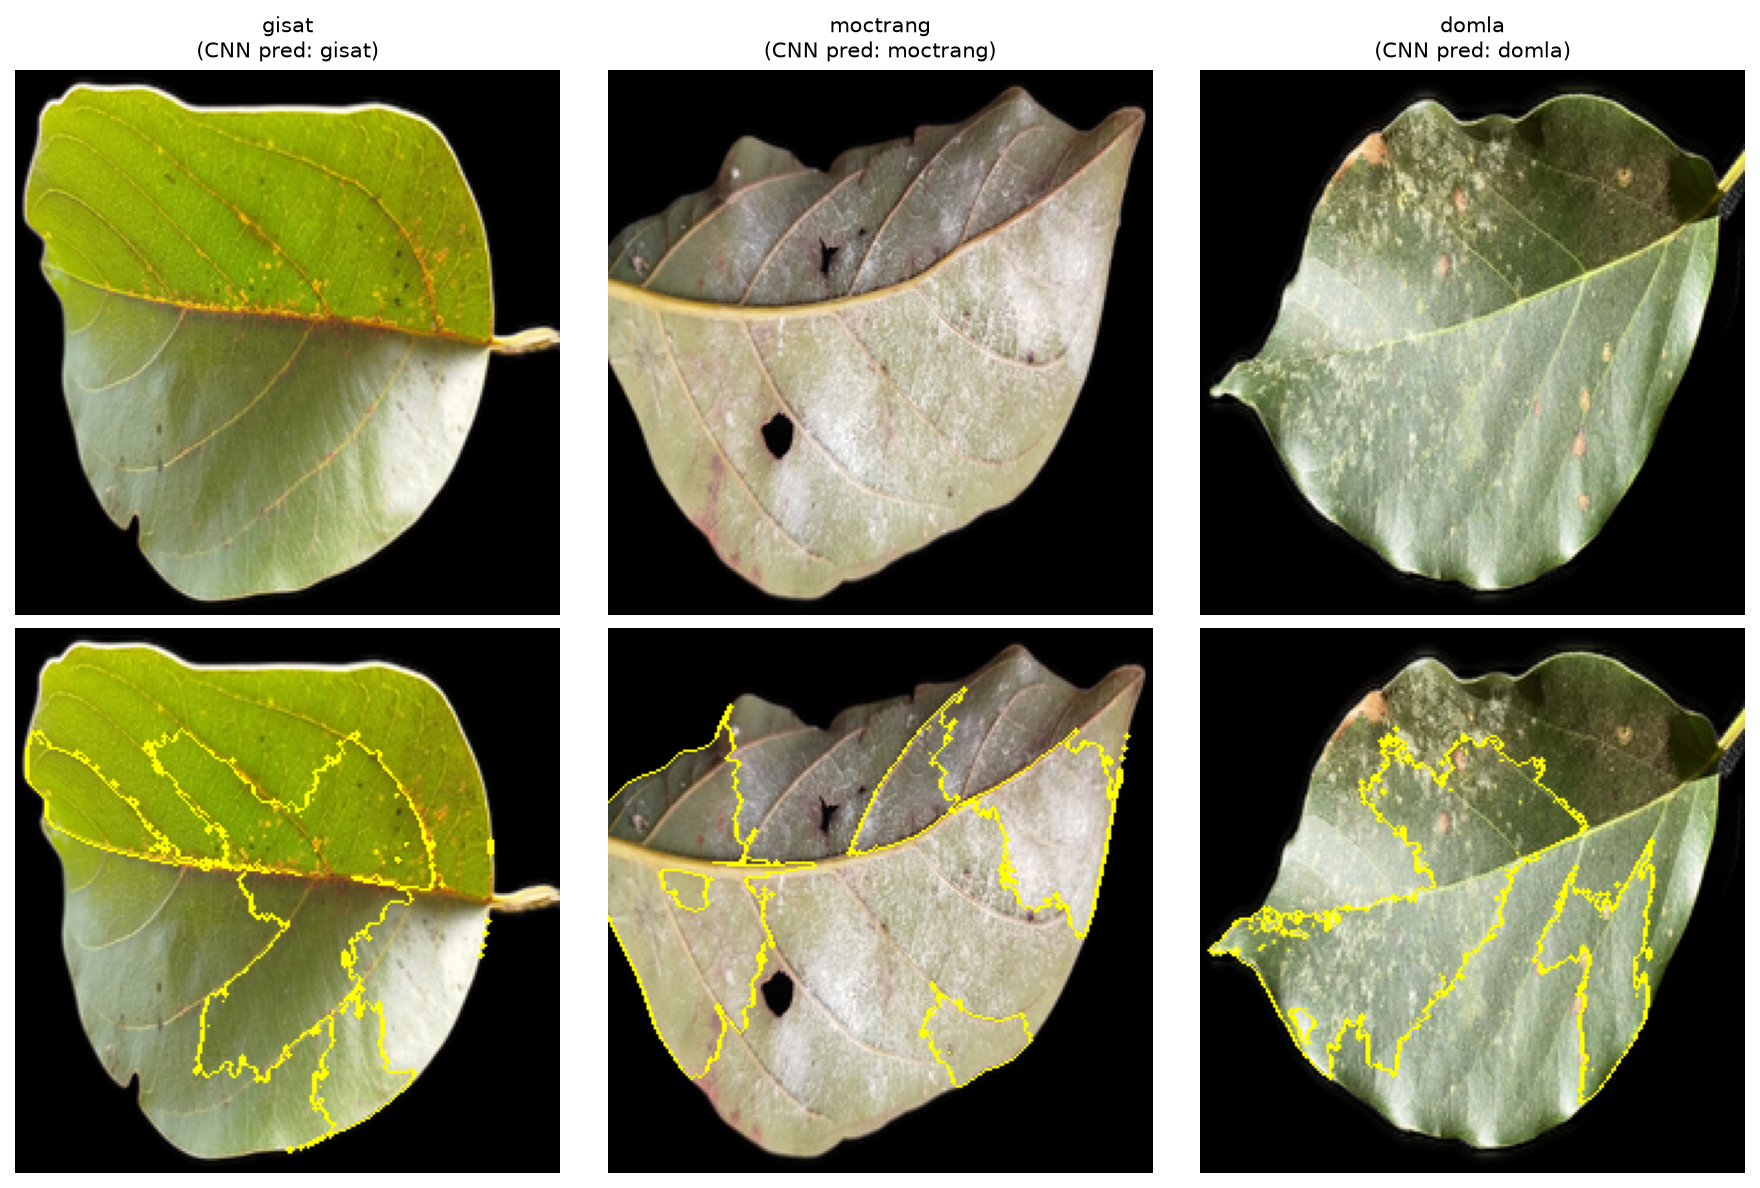
\includegraphics[width=\linewidth]{img/experiments/llm/explain_vlm_showcase.png}
\caption{Three examples of the combined CNN + LIME + VLM explanation pipeline. Top row, original test images; bottom row, LIME overlay (yellow outlines) shown to the VLM alongside the CNN's prediction. Generated explanations are given in Table~\ref{tab:explain_vlm_showcase}.}
\label{fig:explain_vlm_showcase}
\end{figure}

\begin{table}[htbp]
\centering
\caption{VLM-generated explanations for the three examples in Figure~\ref{fig:explain_vlm_showcase}, translated from Vietnamese.}
\label{tab:explain_vlm_showcase}
\small
\begin{tabular}{p{0.12\linewidth} p{0.78\linewidth}}
\toprule
\textbf{Class} & \textbf{Generated visual evidence} \\
\midrule
gisat & ``The CNN's most-attended region is in the middle of the leaf, particularly the area with rust-orange-coloured spots, typically on the underside -- this may be a sign of \textit{gisat}.'' \\
moctrang & ``The estimated region between the two images has many yellow-outlined patches, indicating white powdery spots on the leaf -- the CNN attended most to this region when predicting \textit{moctrang}.'' \\
domla & ``The CNN's most-attended region is near the centre of the leaf, close to the leaf-spot location; the spot's colour and shape resemble the small, round or irregular spots on the leaf surface [that define \textit{domla}].'' \\
\bottomrule
\end{tabular}
\end{table}

This capability is distinct from, and should not be conflated with, using the same VLM output as an automatic error detector. Section~\ref{sec:discussion} and \ref{app:llm} report a separate, secondary analysis of whether the \texttt{supports\_cnn\_diagnosis} judgement can substitute for or complement predictive-entropy-based flagging of likely CNN mistakes, which was \emph{not} successful. The explanation-generation capability demonstrated here is unaffected by that negative result; the pipeline is \emph{capable} of producing a plausible, grounded caption for a prediction, as shown by the curated examples above, though we have not established how often it does so unprompted across the full subset, nor validated the captions against expert judgement rather than an automated proxy. Whether such captions are a reliable enough signal to automatically flag errors without human review is a separate, harder question that Section~\ref{sec:discussion} answers in the negative for this specific use.


\subsection{Few-shot Learning}
\label{subsec:fewshot}

To evaluate the ability of our model to generalise from very few labelled examples – a realistic scenario in agricultural applications where data collection is expensive – we conducted few-shot experiments on the AvocadoLeaf dataset. We compared three approaches, namely (i) standard fine-tuning of the entire classifier on the limited support set (denoted as \texttt{Fine‑tune}), (ii) Prototypical Networks (ProtoNet) using a frozen ConvNeXt‑V2 backbone, and (iii) Relation Networks (RelationNet) with the same frozen backbone.

For each setting, we randomly sampled \(K\) images per class (\(K \in \{1,5,10,20\}\)) from the training set to form the support set, and evaluated on the full test set. Fine‑tune was trained for 50 epochs with early stopping; for ProtoNet and RelationNet we report the mean accuracy and standard deviation over 600 randomly generated episodes (6‑way, \(K\)-shot, 5 query images per class).

The quantitative results are summarised in Table~\ref{tab:fewshot_results}, and a visual comparison is provided in Figure~\ref{fig:fewshot_acc}. Several observations can be made:

\begin{itemize}
    \item \textbf{Fine‑tune suffers from severe overfitting} when only a few samples per class are available. With only 5 shots, it achieves only 16.4\% accuracy, and even with 20 shots it reaches only 28.6\%, indicating that conventional fine‑tuning is not suitable for extreme low‑data regimes.
    
    \item \textbf{Prototypical Networks substantially outperforms fine‑tuning at all shot levels.} Already with 1 shot per class, ProtoNet attains 28.9\% accuracy, which is higher than fine‑tuning with 5 shots (16.4\%). The gap remains large as the number of shots increases. At 5 shots ProtoNet achieves 45.7\% (+29.2 p.p.), at 10 shots 52.3\% (+31.3 p.p.), and at 20 shots 57.4\% (+28.9 p.p.). These results demonstrate that metric‑based few‑shot learning is substantially more effective than fine‑tuning for fine‑grained plant disease classification, even though absolute accuracy remains moderate.
    
    \item \textbf{Relation Networks perform poorly} on this dataset, with accuracy remaining close to the 16.7\% random-chance baseline (16–19\%) across all shot levels and showing no consistent improvement as the number of shots increases (see Figure~\ref{fig:fewshot_acc}). This suggests that the learnable distance metric of RelationNet may overfit to the specific episode composition or that the relation module requires more training data to generalise.
\end{itemize}

Overall, the ProtoNet framework combined with a frozen ConvNeXt‑V2 backbone provides the strongest few‑shot baseline among the three methods evaluated, more than doubling fine‑tuning's accuracy at every shot level tested and reaching 57.4\% accuracy with only 20 labeled images per class. While this is well below the $>$90\% accuracy achieved with the full training set (Table~\ref{tab:arch_compare}), it demonstrates that metric-based few-shot learning is a substantially more data-efficient starting point than fine-tuning for scenarios where data collection is expensive.

\begin{table*}[t]
\centering
\caption{Few-shot classification accuracy (\%) on the test set. Fine‑tune results are from a single training run; ProtoNet and RelationNet results are averaged over 600 random episodes (mean \(\pm\) std).}
\label{tab:fewshot_results}
\begin{tabular}{lcccc}
\toprule
\textbf{Method} & \textbf{1-shot} & \textbf{5-shot} & \textbf{10-shot} & \textbf{20-shot} \\
\midrule
Fine‑tune       & --              & 16.43           & 21.07           & 28.57           \\
ProtoNet        & {\textbf{28.9 ± 8.3}}  & {\textbf{45.7 ± 9.1}}  & {\textbf{52.3 ± 8.8}}  & {\textbf{57.4 ± 9.0}}  \\
RelationNet     & 16.2 ± 5.9      & 18.5 ± 6.3      & 17.5 ± 6.2      & 19.4 ± 6.9      \\
\bottomrule
\end{tabular}
\end{table*}

\begin{figure}[htbp]
\centering
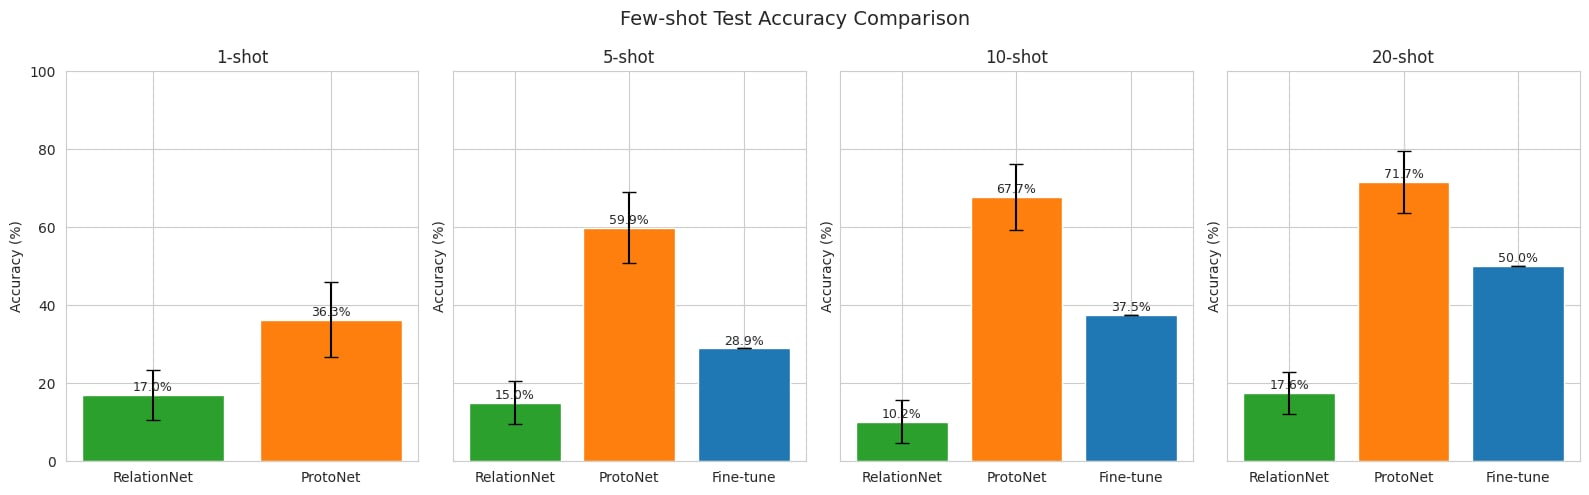
\includegraphics[width=\columnwidth]{img/experiments/fewshot/acc_comparison.jpg}
\caption{Few-shot test accuracy comparison. Error bars represent standard deviation (ProtoNet, RelationNet). Fine‑tune results are single runs.}
\label{fig:fewshot_acc}
\end{figure}




\subsection{Uncertainty Estimation}
\label{subsec:uncertainty}

A high accuracy alone does not guarantee that a model knows when it is unsure. We therefore examine two complementary aspects, calibration and out-of-distribution detection.

\subsubsection{Calibration}

We compute the Expected Calibration Error (ECE) on the validation set. Our baseline softmax model achieves an ECE of 0.0625. This is somewhat above the common threshold of 0.05 used to indicate good calibration, suggesting the model's raw softmax confidence is only moderately well calibrated and would benefit from post-hoc calibration before its confidence scores are used directly in high-stakes decisions.

We apply single-parameter temperature scaling \cite{guo2017calibration}: a scalar $T$ is fit by minimising negative log-likelihood on the validation logits, then used to rescale logits before softmax at inference ($T$ does not change arg-max predictions, so accuracy is unaffected by construction). The fitted temperature is $T=1.274$ ($T>1$ indicates the raw model is overconfident, consistent with the ECE above 0.05). On the validation set this reduces ECE from 0.0625 to 0.0505, essentially at the 0.05 threshold; on the held-out test set, independent of the temperature fit, ECE improves from 0.0311 to 0.0193, clearly within the good-calibration range. Figure~\ref{fig:reliability_diagram} shows the corresponding reliability diagrams. Temperature scaling is a one-parameter, post-training operation with no retraining and negligible inference-time cost, so we recommend it be applied whenever BoVien's raw confidence is surfaced to an end user.

\begin{figure}[htbp]
\centering
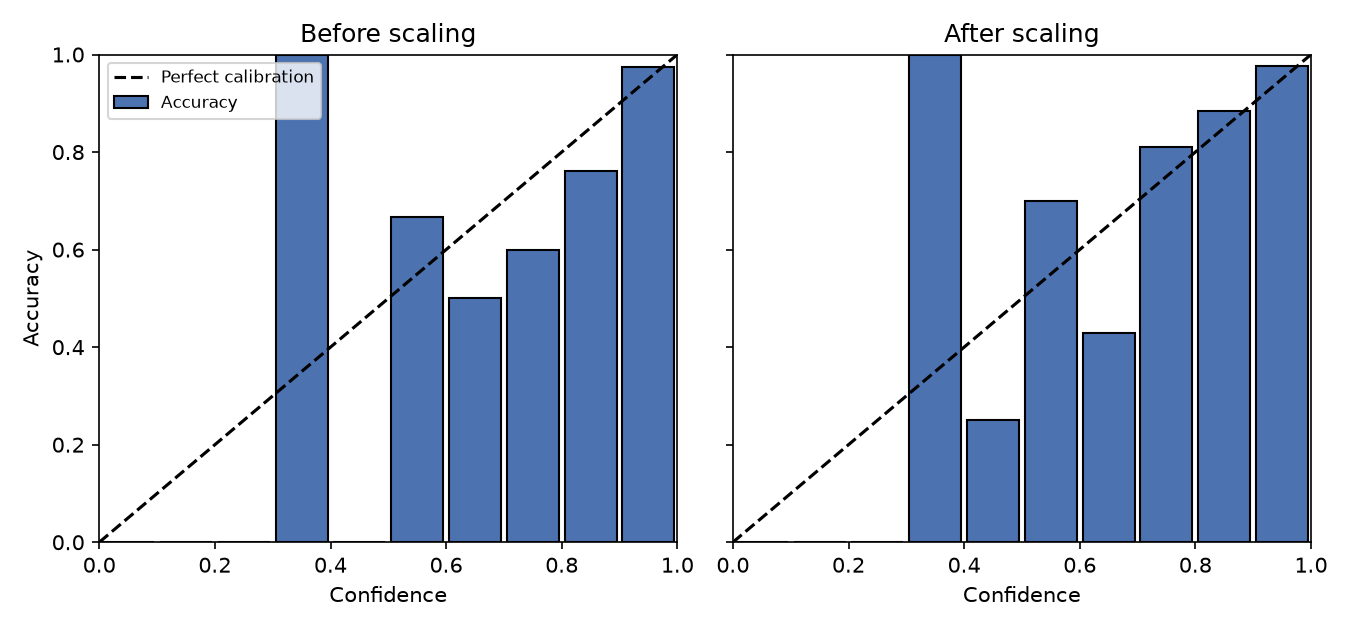
\includegraphics[width=\columnwidth]{img/experiments/calibration/reliability_diagram.png}
\caption{Reliability diagrams (test set, 10 bins) before and after temperature scaling ($T=1.274$). Bars show empirical accuracy per confidence bin; the dashed diagonal is perfect calibration. Some bins are sparsely populated given the 280-image test set, which is why individual bars can look noisy even as the aggregate ECE improves.}
\label{fig:reliability_diagram}
\end{figure}

\subsubsection{Far out of distribution detection}

We collect 200 random images from the internet, including animals, landscapes and objects. These images are completely unrelated to leaves. Using Monte Carlo Dropout with 50 forward passes, we compute the predictive entropy. The area under the ROC curve reaches 0.994, meaning the model almost perfectly separates avocado leaf images from far domain images. The mean entropy for in distribution validation samples is 0.21, while for far OOD samples it is 1.46. This large gap confirms that the model becomes highly uncertain when confronted with entirely irrelevant inputs.

Figure~\ref{fig:far_entropy} shows the entropy histogram for this experiment.

\begin{figure}[htbp]
\centering
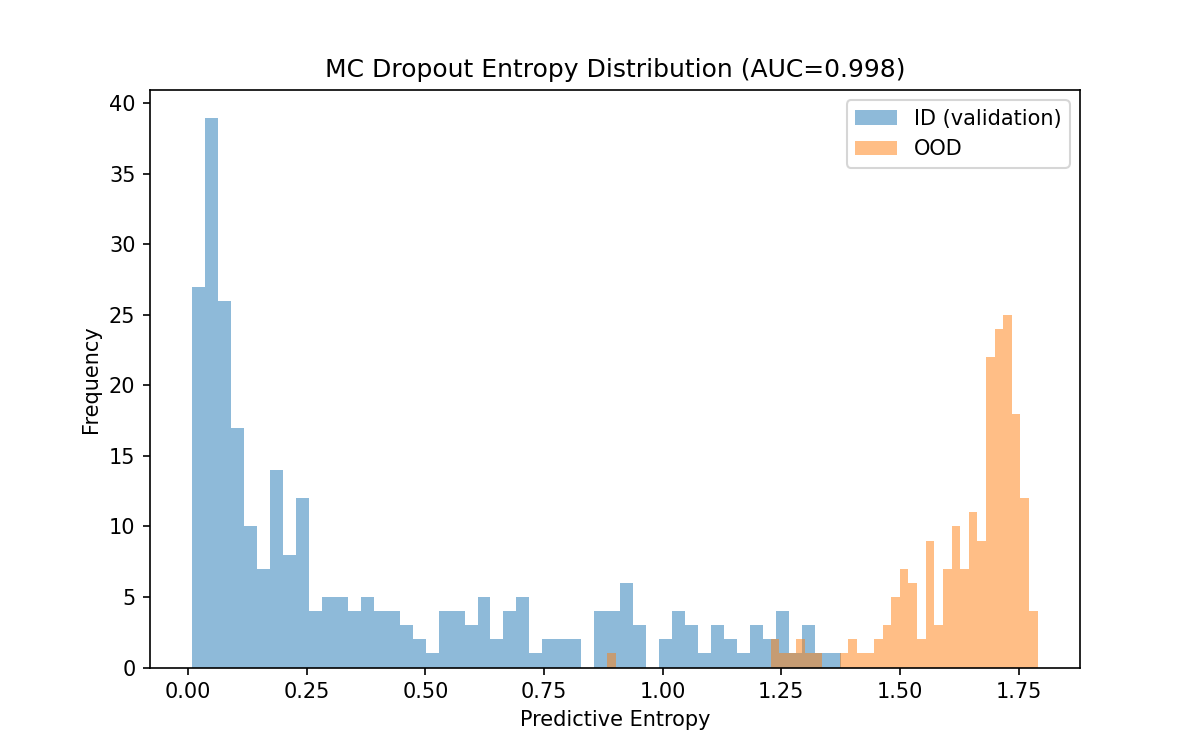
\includegraphics[width=0.49\textwidth]{img/experiments/uncertainty/far_entropy_histogram.png}
\caption{Entropy distribution on far OOD (random internet images). ID samples concentrate at very low entropy, OOD samples at high entropy, with almost no overlap.}
\label{fig:far_entropy}
\end{figure}

\subsubsection{Near out of distribution detection}

A more realistic challenge comes from leaf images of other crop species. We take 200 images from the PlantVillage dataset, containing leaves of tomato, corn and potato. These images still depict leaves but belong to plants that are never seen during training. The model achieves an AUC of 0.985 on this near OOD set, nearly as strong as the far OOD result. The mean entropy for near OOD samples is 1.35, noticeably higher than the 0.21 of the in distribution validation set. This shows that the model's uncertainty is not merely picking up on trivial domain shift (as in the far OOD case) but also distinguishes avocado leaves from visually similar leaves of other crop species.

Figure~\ref{fig:near_entropy} presents the corresponding entropy histogram.

\begin{figure}[htbp]
\centering
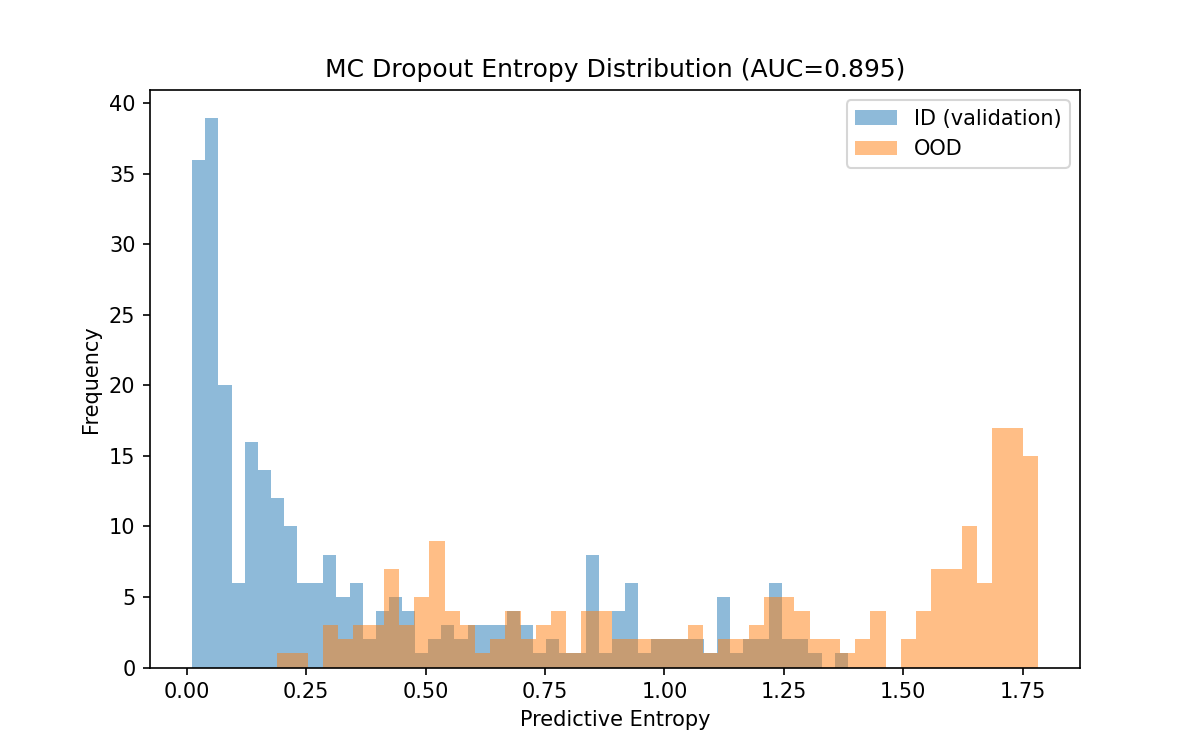
\includegraphics[width=0.49\textwidth]{img/experiments/uncertainty/near_entropy_histogram.png}
\caption{Entropy distribution on near OOD (PlantVillage leaves). ID samples still cluster at low entropy, while near OOD samples shift to high entropy, with only a small overlap, consistent with the AUC of 0.985.}
\label{fig:near_entropy}
\end{figure}

Table~\ref{tab:ood_auc} summarises the OOD detection results.

\begin{table}[htbp]
\centering
\caption{OOD detection AUC using MC Dropout entropy.}
\label{tab:ood_auc}
\begin{tabular}{lcc}
\toprule
\textbf{OOD set} & \textbf{Type} & \textbf{AUC} \\
\midrule
Random internet images & Far OOD & 0.994 \\
PlantVillage leaves & Near OOD & 0.985 \\
\bottomrule
\end{tabular}
\end{table}

\subsection{Cross-dataset Evaluation}
\label{subsec:cross_dataset}

The uncertainty analysis above shows that ConvNeXt‑V2's predictive entropy reliably \emph{flags} domain-shifted inputs when that signal is explicitly used as a detector (Section~\ref{subsec:uncertainty}). This raises a distinct, practically important question. What would happen if a model were deployed \emph{without} that uncertainty gate, simply taking the arg-max class at face value? This section first quantifies that naive-deployment failure mode on off-task images (Section~\ref{subsec:cross_dataset}.1), then reports, in Section~\ref{subsec:cross_dataset}.2, a genuine same-task train-A/test-B evaluation on an independently collected avocado leaf dataset.

\subsubsection{Naive-Deployment Behaviour on Off-Task Inputs}

We reuse the existing far-OOD (random internet images) and near-OOD (PlantVillage tomato/corn/potato leaves) sets from Section~\ref{subsec:uncertainty} to quantify a complementary, and more immediately actionable, failure mode. For each of three models spanning our accuracy/efficiency trade-off (ConvNeXt‑V2, proposed and highest accuracy; MobileNet‑V2, fastest and smallest; MobileOne, edge-specialised and statistically tied accuracy), we run a single deterministic forward pass over both OOD sets and record the arg-max class and its softmax confidence, with no MC-Dropout averaging and no rejection threshold applied.

The three models diverge sharply. ConvNeXt‑V2 is the most conservative, with only 23.5\% of far-OOD and 35.5\% of near-OOD images assigned confidence above 0.5, and essentially none (0.0\% far-OOD, 1.5\% near-OOD) exceeding 0.9. MobileNet‑V2 is the opposite, with 81.5\% of far-OOD and 82.0\% of near-OOD images accepted at confidence $>0.5$, and a striking 29.5\% (far-OOD) and 22.0\% (near-OOD) exceed 0.9 confidence despite depicting no avocado leaf at all. MobileOne sits in between (62.0--71.5\% at $>0.5$, 4.0--12.0\% at $>0.9$). Figure~\ref{fig:cross_dataset_acceptance} summarises the acceptance rate at the 0.5 threshold for all three models and both OOD sets; Table~\ref{tab:cross_dataset_predictions} reports the full breakdown, including which classes the rejected mass is (incorrectly) attributed to.

\begin{figure}[htbp]
\centering
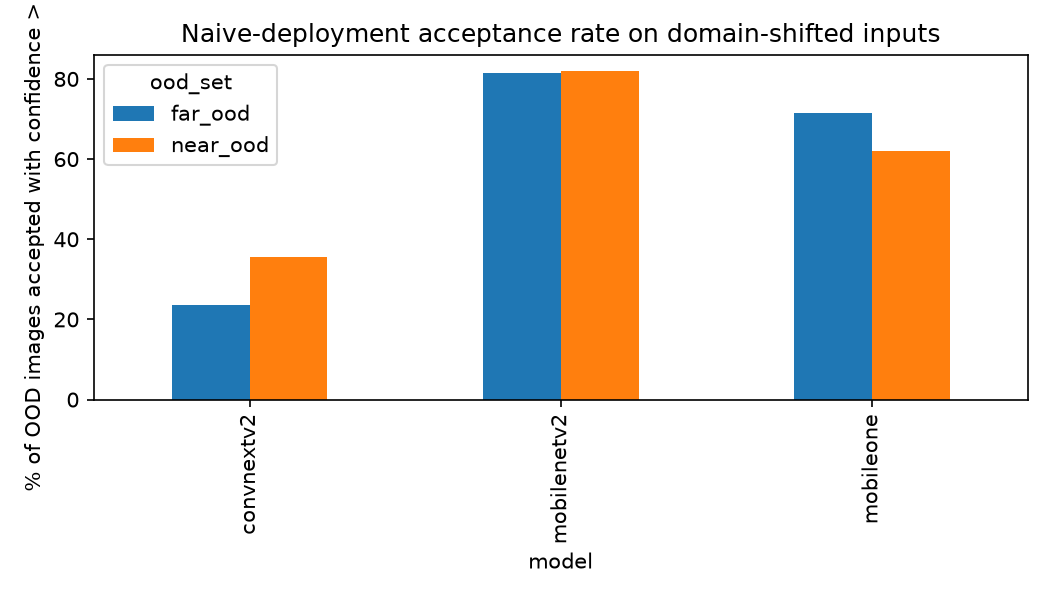
\includegraphics[width=\columnwidth]{img/experiments/cross_dataset/confidence_by_class.png}
\caption{Percentage of out-of-domain images (far-OOD, random internet images; near-OOD, PlantVillage leaves) that a naive arg-max deployment, with no uncertainty gate, would accept at confidence $>0.5$, for each of the three demo models.}
\label{fig:cross_dataset_acceptance}
\end{figure}

\begin{table*}[t]
\centering
\caption{Naive-deployment behaviour on domain-shifted inputs (no uncertainty gate; single forward pass, arg-max class).}
\label{tab:cross_dataset_predictions}
\small
\begin{tabular}{lccc}
\toprule
\textbf{Model} & \textbf{OOD set} & \textbf{Mean conf.} & \textbf{\% conf.$>$0.5 / $>$0.9} \\
\midrule
ConvNeXt‑V2  & Far OOD  & 0.422 & 23.5 / 0.0 \\
ConvNeXt‑V2  & Near OOD & 0.462 & 35.5 / 1.5 \\
MobileNet‑V2 & Far OOD  & 0.731 & 81.5 / 29.5 \\
MobileNet‑V2 & Near OOD & 0.700 & 82.0 / 22.0 \\
MobileOne    & Far OOD  & 0.654 & 71.5 / 12.0 \\
MobileOne    & Near OOD & 0.576 & 62.0 / 4.0 \\
\bottomrule
\end{tabular}
\end{table*}

This result reframes the accuracy/efficiency trade-off of Section~\ref{subsec:arch_compare}. ConvNeXt‑V2's advantage over MobileNet‑V2 and MobileOne is not only higher in-distribution accuracy (92.14\% vs. 87.14\% and 91.43\% respectively) but also substantially safer behaviour under distribution shift, i.e. it degrades towards low-confidence, easily-rejectable predictions rather than confidently misclassifying unrelated inputs. Practically, this means that if a lighter model such as MobileNet‑V2 is chosen for a resource-constrained deployment on the strength of its speed and size (Section~\ref{subsec:efficiency}), the entropy-based uncertainty gate already validated in Section~\ref{subsec:uncertainty} is not optional but necessary. Without it, roughly four in five domain-shifted inputs would be silently and confidently misdiagnosed as a specific avocado disease.

\subsubsection{Real Cross-Domain Evaluation (Train A, Test B)}
\label{subsec:real_cross_domain}

Section~\ref{subsec:cross_dataset}.1 characterises behaviour on off-task inputs, but does not answer the question that matters most for external validity: trained only on AvocadoLeaf (domain A, collected first-hand in Vietnam), does BoVien still recognise avocado leaf disease on leaves it has never seen, collected independently, in a different country, under a different camera and background? K-Kotagiri \cite{kotagiri2024avocado} (Table~\ref{tab:dataset_comparison}), a 435-image, healthy/diseased-labelled avocado leaf dataset collected in Tamil Nadu, India, lets us test this directly for the first time. Because Kotagiri provides only binary labels, BoVien's 6-way prediction is collapsed to binary (\textit{binhthuong} $\to$ healthy, the other five disease classes $\to$ diseased) for this comparison; a same-task but coarser test than the full 6-class problem. To isolate genuine domain shift in leaf and disease appearance from a simple background-format mismatch, every Kotagiri image is passed through the same background-removal preprocessing (\texttt{rembg}-based foreground segmentation, crop, resize to $224\times224$) used to build \texttt{data/processed/} for AvocadoLeaf itself, rather than fed to the model on its original concrete/stone background.

\begin{table}[htbp]
\centering
\caption{Zero-shot cross-domain evaluation: BoVien trained on AvocadoLeaf (domain A), evaluated with no retraining on both its own test set and K-Kotagiri (domain B), both collapsed to binary (healthy vs. diseased) for a like-for-like comparison.}
\label{tab:real_cross_domain}
\small
\begin{tabular}{lcc}
\toprule
\textbf{Metric} & \textbf{Domain A} & \textbf{Domain B} \\
\midrule
n                 & 280     & 435 \\
Accuracy          & 98.57\% & \textbf{60.00\%} \\
Precision (dis.)  & 0.987   & 0.627 \\
Recall (dis.)     & 0.996   & 0.481 \\
Macro F1          & 0.976   & 0.594 \\
\bottomrule
\end{tabular}
\end{table}

The drop is severe: accuracy falls 38.6 percentage points (98.57\% $\to$ 60.00\%), and recall on the diseased class collapses to 48.1\%, meaning BoVien misses over half of the genuinely diseased Kotagiri leaves, barely better than chance on this near-balanced (219 healthy / 216 diseased) binary problem. This confirms that the strong in-distribution accuracy reported throughout this paper (Section~\ref{subsec:arch_compare}) does not, by itself, imply robustness to a truly independent collection site, and is consistent with the OOD-detection results above: whatever ConvNeXt-V2 has learned generalises well to inputs like the ones it was trained on, but far less well to a genuinely new domain within the same task.

Following the fallback strategy motivated by this gap, we test whether a handful of labelled Kotagiri examples can adapt the model without retraining it. Using BoVien's fine-tuned backbone as a frozen feature extractor, we compute a class prototype (feature centroid) from $k$ randomly drawn support images per class and classify every remaining Kotagiri image by nearest prototype (ProtoNet-style; Section~\ref{sec:experiments} follows the same recipe as the within-domain few-shot evaluation in Section~\ref{subsec:fewshot}), averaged over 200 random supports per $k$ for stability.

\begin{figure}[htbp]
\centering
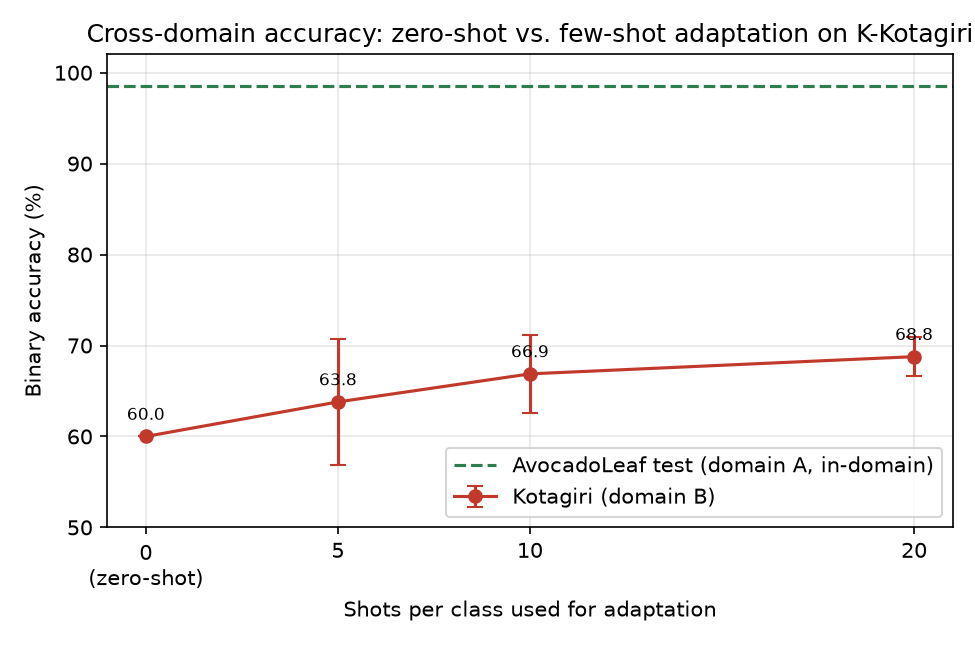
\includegraphics[width=\columnwidth]{img/experiments/cross_dataset/kotagiri_fewshot_recovery.png}
\caption{Binary accuracy on K-Kotagiri: zero-shot (BoVien's own classifier head) versus few-shot nearest-prototype adaptation using BoVien's fine-tuned backbone as a frozen feature extractor, at 5/10/20 labelled Kotagiri images per class (200 random supports each; error bars are $\pm 1$ std). The dashed line is BoVien's in-domain (AvocadoLeaf test set) binary accuracy.}
\label{fig:kotagiri_fewshot}
\end{figure}

Few-shot adaptation helps but does not close the gap: accuracy rises from 60.00\% (zero-shot) to 63.80\% $\pm$ 6.91\% at 5 shots, 66.88\% $\pm$ 4.26\% at 10 shots, and 68.78\% $\pm$ 2.16\% at 20 shots per class, a monotonic and increasingly stable improvement, but still 30 points short of the 98.57\% in-domain accuracy. Practically, this means that a handful of labelled examples from a new deployment site is worth collecting and does measurably help, but is not, on its own, a substitute for either a larger site-specific labelled set or a properly retrained/fine-tuned model; see Section~\ref{sec:discussion} for how this qualifies the paper's edge-deployment and generalisation claims.

\subsection{Real-time Inference under Realistic Conditions}
\label{subsec:realtime_demo}

The architecture comparison in Section~\ref{subsec:arch_compare} reports GPU inference latency measured on batched, pre-processed test images. To obtain a first read on latency and prediction behaviour under conditions closer to field use, we built a real-time demo that captures frames live from a laptop webcam, runs them through one of the three models from Section~\ref{subsec:cross_dataset} (switchable at runtime), and overlays the predicted class, confidence, and per-frame latency. Leaf photographs are presented to the camera on a phone screen, and every frame's prediction, confidence, and latency are logged to CSV.

% TODO (future work), Populate this subsection with the numbers from an actual
% webcam session once run (see source/src/experiments/realtime_demo/README.md
% for the exact procedure and the command to summarise the logged CSV into
% mean/median latency, FPS, and mean confidence per model). The script itself
% has been implemented and smoke-tested against static leaf images (confirming
% model loading, preprocessing, overlay rendering, and CSV logging all work
% correctly) but has not yet been run against a live camera and phone, so no
% numbers are reported here yet.
\begin{table*}[t]
\centering
\caption{Real-time inference latency and prediction confidence on a laptop webcam, measured over a live session (phone-displayed leaf images). \emph{This measures host-machine latency, not true embedded-hardware latency; see Limitations, Section~\ref{sec:discussion}.}}
\label{tab:realtime_demo}
\begin{tabular}{lccc}
\toprule
\textbf{Model} & \textbf{Mean latency (ms)} & \textbf{FPS} & \textbf{Mean confidence} \\
\midrule
ConvNeXt‑V2  & -- & -- & -- \\
MobileNet‑V2 & -- & -- & -- \\
MobileOne    & -- & -- & -- \\
\bottomrule
\end{tabular}
\end{table*}
